\begin{problem}{四星珠}{四星珠.in}{四星珠.out}{2.5 seconds}


一棵树,一棵树

彼此孤离地兀立着

风与空气

告诉着他们的距离

但是在泥土的覆盖下

他们的根伸长着

在看不见的深处

他们把根须纠缠在一起

木工本的诗情在于诗意地砍树。一棵树由$n$个节点与$n-1$条边组成,树上的任意节点间可以互相到达。

如果一个节点的度为偶数,则可以被诗意地砍掉,并且所有与他相连的边都会消失。

是否存在一种方案,小本可以诗意地砍完整棵树?

\InputFile

第一行一个整数$n\ (1\le n\le 2\times 10^5)$表示节点数量。

第二行$n$个整数$p_1,p_2,\cdots,p_n\ (0\le p_i\le n$ 且 $p_i\ne i)$,如果$p_i\ne 0$,则表示节点$i$和节点$p_i$之间有边。

数据保证存在且仅存在1个0,且构成一棵合法的树。

\OutputFile

如果存在一种方案满足条件,输出"YES",并换行按顺序输出被砍掉的节点的编号。

如果不存在这样的方案,输出"NO"。

如果有多种方案满足条件,输出任意一种。

\Example

\begin{example}
\exmp{
5
0 1 2 2 1
}{
YES
1 2 3 4 5
}%
\end{example}
\\
\begin{minipage}[b]{0.3\linewidth}
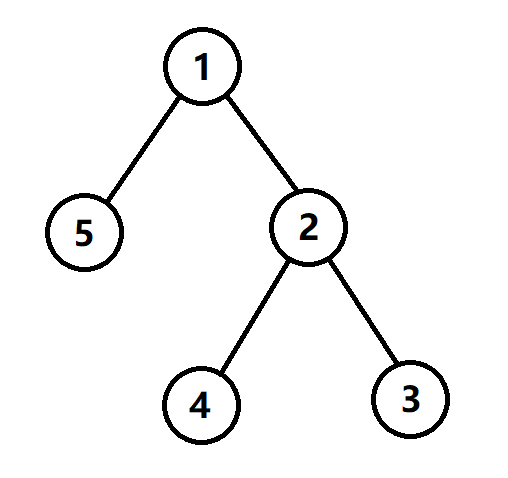
\includegraphics[width=0.7\textwidth]{pics/D.png}
\end{minipage}
\hfill
\begin{minipage}[b]{0.7\linewidth}

对于样例,5个点的度初始为2, 3, 1, 1, 1。

砍掉节点1后,5个点的度为0, 2, 1, 1, 0。

砍掉节点2后,所有点的度均为0。
\end{minipage}
\end{problem}
